\documentclass[11pt,a4paper]{article}

\usepackage{a4wide}
\usepackage{times}
\usepackage[utf8]{inputenc}
\usepackage{graphicx}
\usepackage{subcaption}
\usepackage[square,sort,comma,numbers]{natbib}
\usepackage{float}
\usepackage{booktabs}
\usepackage{amsmath}


\begin{document}

\title{Large Scale Data Exploration with R}
\author{Ashraf, Shawon}
\date{26 June, 2020}

\maketitle


\section{Norms}

\subsection{Dataset}

\paragraph{}
For this data exploration project, I have used the Norms dataset presented by Brysbaert et al. \cite{brys} which contains the concreteness ratings for 40 thousand generally known English word lemmas. According to the authors, concreteness is the measurement of the concept a word demotes to an entity. The concept of concreteness of words came Paivio’s dual-coding theory \cite{paivio} which states that concrete words are easier to recall and activate in memory compared to non concrete words. Also,  Schwanenflugel et al. \citep{schwanenflugel} presented that concrete words are easier to recall because of the supporting memory context imposed by the words on entities to the degree abstract words can not. Vigliocco et al. \cite{vigliocco_vinson_lewis_garrett_2004} and Andrews et al. \cite{andrews_vigliocco_vinson_2009} presented a semantic theory which states that the learning process of words are more based on direct experience of the learners.

\paragraph{}
The authors based their presentation of the Norms based on Connell et al. \cite{connell} which states that despite words being learnt on direct experiences, the existing concreteness ratings were too much focused on visual perception whereas Lynott et al. found that the concreteness ratings were correlated not only on visual perception but also on touch and smell. The overcome the limitations of the existing datasets, the authors came up with the dataset in use which was collected by asking English speakers to rate the concreteness of the words based on their knowledge on them.

\paragraph{}
The Norms dataset consist of 8 columns :
\begin{enumerate}
	\item Word
	\item Whether the word is a Bigram or not
	\item Mean concreteness rating
	\item Standard deviation of the concreteness ratings
	\item Number of persons not knowing the word
	\item Total number or persons rating words
	\item Percentage of persons knowing the word
	\item SUBTLEX-US frequency count of the word \cite{brysbaert_new_2009}
\end{enumerate}

\subsection{Variables chosen}

\begin{itemize}
	\item Mean concreteness rating
	\item Standard deviation of the concreteness ratings
	\item Percentage of persons knowing the word
\end{itemize}


\section{Preprocessing}
\paragraph{}
The provided datasets were processed using unix tools such as awk, cat, etc.

\subsection{Windows}
\begin{itemize}
	\item POS : NN
	\item Frequency count : Greater than 20000
	\item Excluded characters : ":::"
	\item The processed output was converted to a csv file for importing into R
	\item Reduced from 49776264 items to 11046 after processing
\end{itemize}

\subsection{Frequencies}
\begin{itemize}
	\item POS : NN
	\item Frequency count : Greater than 5000
	\item The processed output was converted to a csv file for importing into R
	\item Reduced from 326775 items to 59947 after processing
\end{itemize}


\subsection{Norms}
\paragraph{}
The Norms dataset was already provided in .xlsx format and did not need preprocessing via Unix tools. Norms with words having the POS tag Noun were extracted using R function `subset` during analysis.


\section{Descriptive Statistics and plots of Norms}

\subsection{Mean Concreteness}
\paragraph{}
The minimum mean concreteness value is 1.07 and the variable ranges from 1.07 to 5.0. Median and mean values are 3.66 and 3.53 respectively. While the first quartile ranges to 2.67, the third quartile peaks at 4.46.

\begin{figure}[H]
  \centering
  \begin{subfigure}[b]{0.4\linewidth}
    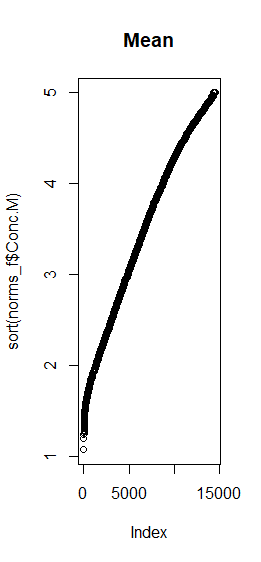
\includegraphics[width=\linewidth]{images/mean_norm.png}
  \end{subfigure}
  \begin{subfigure}[b]{0.4\linewidth}
    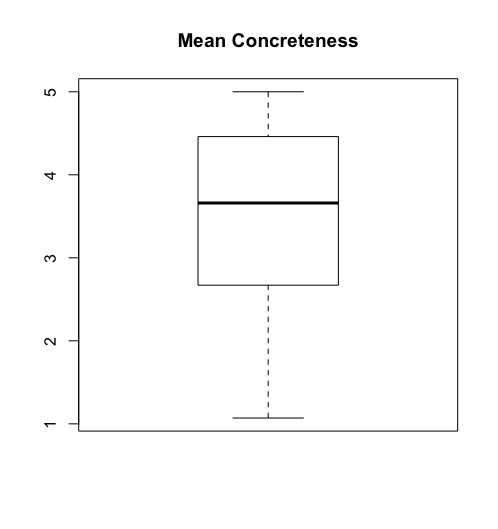
\includegraphics[width=\linewidth]{images/box_concm.png}
  \end{subfigure}
  \caption{Mean concreteness}
  \label{fig:concm}
\end{figure}



\subsection{Standard Deviation of Concreteness}
\paragraph{}
The minimum value is 0 and the variable ranges from 0 to 1.890. Median and mean values are 1.2 and 1.109 respectively. While the first quartile ranges to 0.920, the third quartile peaks at 1.370.

\begin{figure}[H]
  \centering
  \begin{subfigure}[b]{0.4\linewidth}
    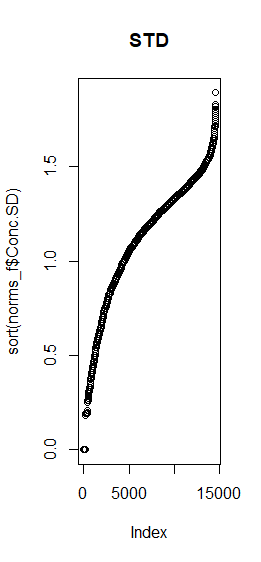
\includegraphics[width=\linewidth]{images/std_norm.png}
  \end{subfigure}
  \begin{subfigure}[b]{0.4\linewidth}
    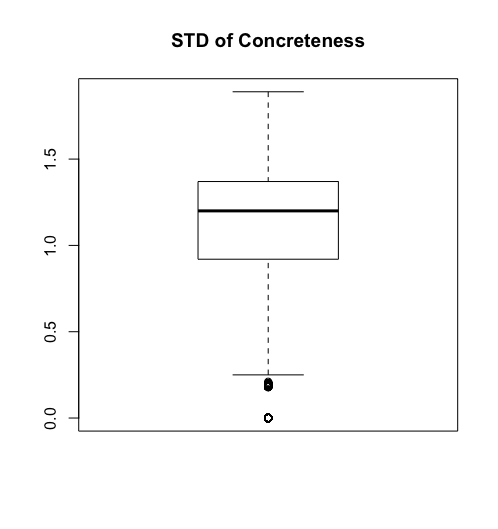
\includegraphics[width=\linewidth]{images/box_conc_std.png}
  \end{subfigure}
  \caption{Standard deviation of concreteness}
  \label{fig:concsd}
\end{figure}



\subsection{Percentage Known}
\paragraph{}
The minimum value is 0.8462 and the variable ranges from 0.8462 to 1. Median and mean values are 1 and 0.9720 respectively. While the first quartile ranges to 0.9630, the third quartile peaks at 1.

\begin{figure}[H]
  \centering
  \begin{subfigure}[b]{0.4\linewidth}
    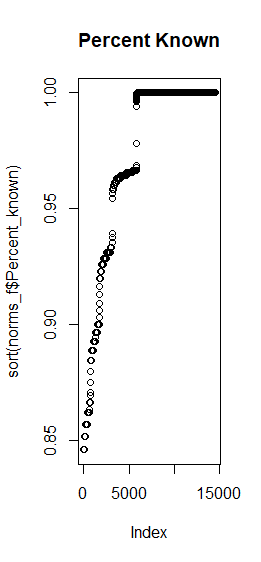
\includegraphics[width=\linewidth]{images/perc_known_norm.png}
  \end{subfigure}
  \begin{subfigure}[b]{0.4\linewidth}
    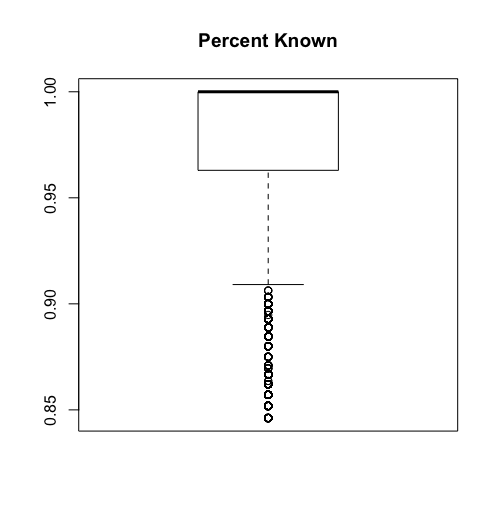
\includegraphics[width=\linewidth]{images/box_perc_known.png}
  \end{subfigure}
  \caption{Percentage Known}
  \label{fig:pk}
\end{figure}

\section{Hypothesis Testing Methods}

\subsection{The ratings of the chosen variables are related to each other across the target words}
\paragraph{}
The Windows dataset contains multiple instances of the same dataset as it also contains the context word related to each of them. To minimize them, the means of context frequency and lmi for the words taken and put into a vector. Then norms for the target words were loaded to run correlation on based on the norm variables. For correlation the lsr\cite{lsr} package was used.

\paragraph{}
The correlation results were as follows:

\begin{table}[H]
\centering
\begin{tabular}{@{}llll@{}}
\toprule
target    & mean   & std    & percent known \\ \midrule
frequency & -0.029 & 0.040  & 0.010         \\
lmi       & 0.033  & -0.008 & 0.020         \\ \bottomrule
\end{tabular}
\end{table}

\subsection{The target ratings in the norms are related to target corpus frequency}
\paragraph{}
For this hypothesis, norms were first loaded for the target words and then their correlation was measured. The result of the correlation was the following:

\begin{table}[H]
\centering
\begin{tabular}{@{}llll@{}}
\toprule
target & mean   & std   & percent known \\ \midrule
freq   & -0.008 & 0.016 & -0.013       \\ \bottomrule
\end{tabular}
\end{table}

\subsection{The target ratings in the norms are related to the semantic diversity of their distributional nearest neighbours}

\begin{itemize}
	\item Target words and their norms were loaded into vectors
	\item Frequency and lmi of the target words were normalized
	norm(x)
	\item The processed output was converted to a csv file for importing into R
	\item Reduced from 326775 items to 59947 after processing
\end{itemize}


% Bibliography:

\bibliography{refs}
\bibliographystyle{ieeetr}


\end{document}


%% --- END OF FILE